\setcitestyle{numbers,open={[},close={]}}

Having developed a method and the means to implement screening calculations, ELNES are calculated for three common lithium compounds with a variety of properties; metallic lithium, LiF, and  $\mathrm{Li_2O}$.  A mixed compound obtained after observing beam damage on LiF during a transformation into metallic lithium is also analyzed and discussed.  Following results from the individual cases the overall effectiveness and applicability of the method is discussed.




\section{Lithium Oxide}

 $ \mathrm{Li_2O} $ is investigated first and screening calculations are performed as described in Section \ref{implementation}.   After the initial two calculations, the electron density around the excited lithium atom is plotted for each, before and after insertion of a core hole, see Fig \ref{Li2O_contour}.  \\

\begin{figure}
	\centering
	\includegraphics[width=0.5\textwidth]{Li2Ocontour_plot}
	\caption{Effect of introducing a core hole in $ \mathrm{Li2O} $.  (a) no hole crystal.  (b) Crystal with hole on starred lithium atom, inducing a response from the valence electrons.  Contour lines on a logarithmic scale. }
	\label{Li2O_contour}
\end{figure}

The density plots clearly show valence electrons in the material being attracted to the excited atom. This response in the electron density indicates that core hole screening should have a noticeable effect on the final states.  Additionally, the closest unexcited lithium atom in the density plot is largely unaffected by the core hole, in agreement with the supercell size being sufficient to isolate core holes.  Calculating the difference in electron occupancy shows a decrease of 0.88 electron in the basin of the excited lithium atom.  This decrease is smaller then would be expected in the no screening limit, and according to Eq. \ref{final_eq} indicates that the hole is 12\% screened.  A third calculation is performed using a correspondingly decreased hole size to obtain a final spectra.  The K edge ELNES from all three simulations are compared to experiment in Fig \ref{Li2O_three}.  \\

In comparison to experiment, the full hole provides good agreement, as previously predicted in the literature \cite{mauchamp_ab_2006}. However, the screened hole provides a superior result, which can be emphasized by measuring the ratio of the two peaks at $\sim$55eV and $\sim$58 eV.  A quantitative comparison of the values, presented in Table \ref{ratio}, reveals a dramatic improvement, decreasing the error in the peak ratio, from 20\% to  6\%.  

\begin{table}[H]
	\centering
		\caption{The ratio of intensities in the $\mathrm{Li_2O}$ spectra between the two peaks at 55 eV and 58 eV.  Errors were calculated relative to experiment.   }
	
	\begin{tabular}{ccc}
		& Ratio & Error \\
		\hline
		Experiment & 0.71 & -  \\
		Full Hole & 0.85 & 20\%  \\
		Screened Hole & 0.66 & 6\%  \\
		
	\end{tabular}
\label{ratio}
\end{table}




\begin{figure}
	\centering
	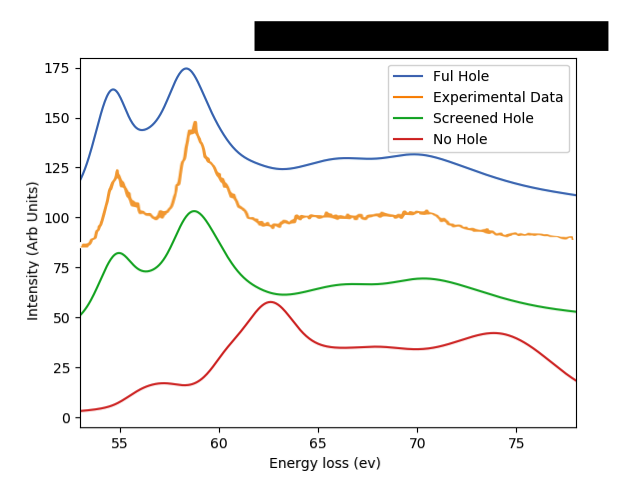
\includegraphics[width=0.65\textwidth]{Li2O_three}
	\caption{Lithium K edge of $ \mathrm{Li_2O} $ from the three calculations taken with varying degrees of core hole. }
	\label{Li2O_three}
\end{figure}

\section{Metallic Lithium}
Metallic lithium has been predicted to exhibit no core hole effects due to a large degree of valence screening \cite{rez_theory_2008}. A density plot supports this notion, revealing that core  holes attract a large number of neighbouring valence electrons, see Fig \ref{Li_countours}.  The response to the excited atom is more aggressive than in $ \mathrm{Li_2O} $, implying a stronger screening impact.  Calculating the screening factor  reveals that the lithium core hole is  $ \sim$41\% screened, larger than in $ \mathrm{Li_2O} $, but less than the full screening predicted in literature. 
\\


\begin{figure}
	\centering
	\includegraphics[width=0.75\textwidth]{Li_contours}
	\caption{Electron density map of metallic lithium, before (a) and after (b) introduction of a core hole on the starred atom.  The contours are on equal logarithmic scales.}
	\label{Li_countours}
\end{figure}




\begin{figure}
	\centering
	\begin{subfigure}{0.45\textwidth}
		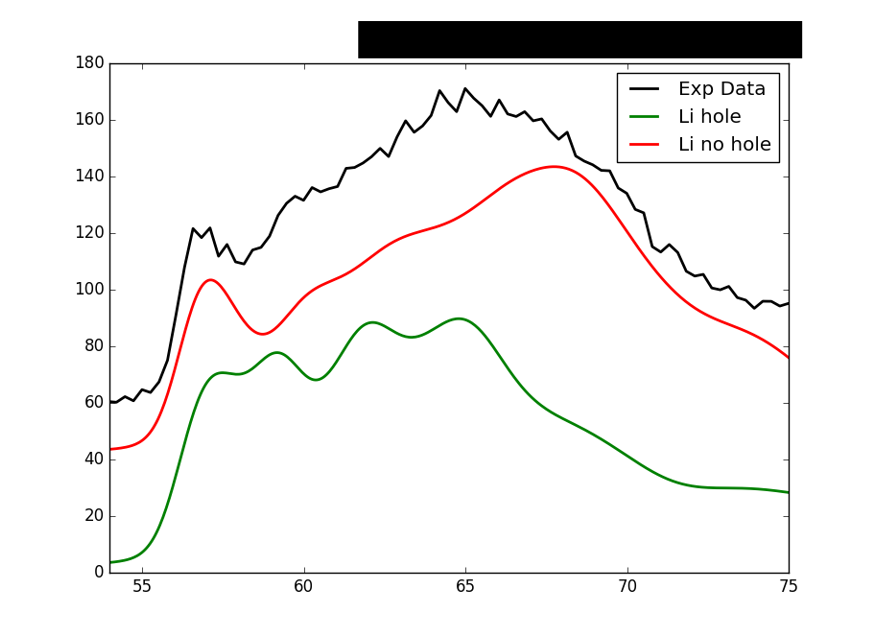
\includegraphics[width=1.1\textwidth]{Li_two}
	\end{subfigure}
	\hspace{-0.01cm}
	\begin{subfigure}{0.45\textwidth}
		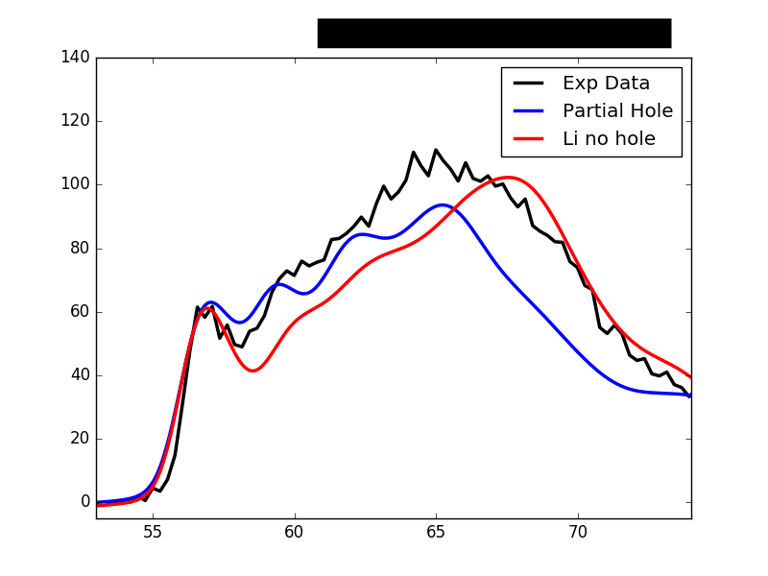
\includegraphics[width=1.1\textwidth]{Li_comparisson}
	\end{subfigure}

	\caption{Lithium K edge of Li from the three calculations taken with varying degrees of core hole. On the left, the full and no hole results are presented, on the right the screened hole spectrum is compared to the no hole spectrum, both normalized to the experimental result at 56 eV. No vertical offset is applied on the right hand graph to better illustrate the differences between the spectra. }
	\label{Li_spectra}
\end{figure}


A comparison of the various core hole cases with experimental spectra is presented in Fig \ref{Li_spectra}. The literature again predicts the superior agreement between full hole and no hole, but both are inferior to the screened hole result.  Of particular note is the small peak located at $ \sim$58 eV, which is underestimated, in the no hole spectra, overestimated in the full hole, and correctly accounted for in the screened case.  The only moderate (41\%) screening goes against common convention in the literature that metals do not exhibit core hole effects.  Other cases of metals requiring core holes have been previously highlighted such as the copper L$_3$ edge and the significant improvements observed with lithium suggest that screened core holes should be included or at least calculated in all cases \cite{hebert_improvement_2003}.  It should be noted that lithium's lack of core electron screening may be contributing to larger core hole effects, which would be lessened for deep core states in heavier elements. 

\section{Lithium Fluoride}
LiF has been one of the more published EELS results for lithium and simulations have obtained good agreement with a full core hole approximation \cite{gao_theory_2008, mauchamp_ab_2006}.  A qualitative probe of the electron density after introducing a core hole reveals lesser effects than observed in Li and $ \mathrm{Li_2O} $, see Fig \ref{LiF_countours}.  The introduction of a hole produces minor responses from the electron density, and these are largely limited to slight distortions in the fluorine electron clouds. Additionally, despite the loss of a core electron, the density around the excited lithium atom retains much of its initial form. The minimal effect of introducing a core hole is reflective of fluorine's high electronegativity and the ionic nature of LiF which ``freezes" all of the electrons in place and minimizes valence electron screening.  This effect is confirmed by calculating the screening coefficient which was determined to be zero in this case. Consequently, LiF represents the no screening case of Eq. \ref{density_calc} and the full hole spectra can be taken as the final spectrum.  Plotting the spectra against experiment confirms that a full hole does indeed produce good agreement, Fig \ref{LiF_spectra}.  The lack of screening in LiF also explains the good results obtained previously in literature when using only a full hole.  It also supports the theory that inserting a full hole can be sufficient in the case of strong insulators, although again, lithium's lack of core electron screening may be contributing to this result.

\begin{figure}
	\centering
	\includegraphics[width=1\textwidth]{LiF_countours}
	\caption{Electron density map of LiF, before (a) and after (b) introduction of a core hole on the starred atom.  The contours are on equal logarithmic scales.}
	\label{LiF_countours}
\end{figure}

\begin{figure}
	\centering
	\includegraphics[width=0.5625\textwidth]{LiF_colour}
	\caption{Lithium K edge of LiF from the two calculations taken with varying degrees of core hole. }
	\label{LiF_spectra}
\end{figure}



\section{Li-LiF Mixture}
The full importance of including screening in core hole calculations is demonstrated when investigating a mixed phase crystal.  When obtaining the spectra for LiF, a transformation to metallic lithium is observed, due to the beam damage.   During this transformation, an acquired intermediate spectra displays both LiF and metallic lithium components.  To investigate the transformation, a linear combination of the spectra from metallic lithium and LiF is compared to the experimental result, see Fig \ref{mix-screened}.  The good agreement obtained here supports both the inclusion of screening in metallic lithium and that the sample contains only metallic lithium and LiF, with no intermediate phases or contamination.  The importance of screening is highlighted in Fig \ref{mix-unscreened}, where the no hole lithium spectra is used, resulting in a  fit that fails to reproduce the peak at 59eV.  This unaccounted for peak would prevent such an  analysis from confirming the purity of the sample and of the mixture.  



\begin{figure}
	\centering
	\begin{subfigure}{0.45\textwidth}
		
		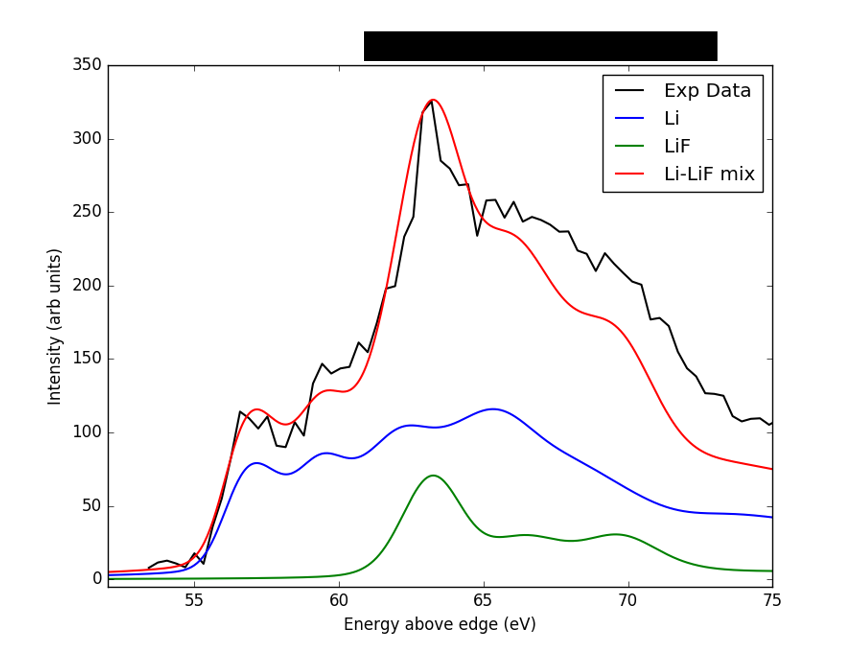
\includegraphics[width=1.1\textwidth]{Li-Lif_colour}
		\caption{}
		\label{mix-screened}
	\end{subfigure}
\hspace{-0.01cm}
	\begin{subfigure}{0.45\textwidth}
		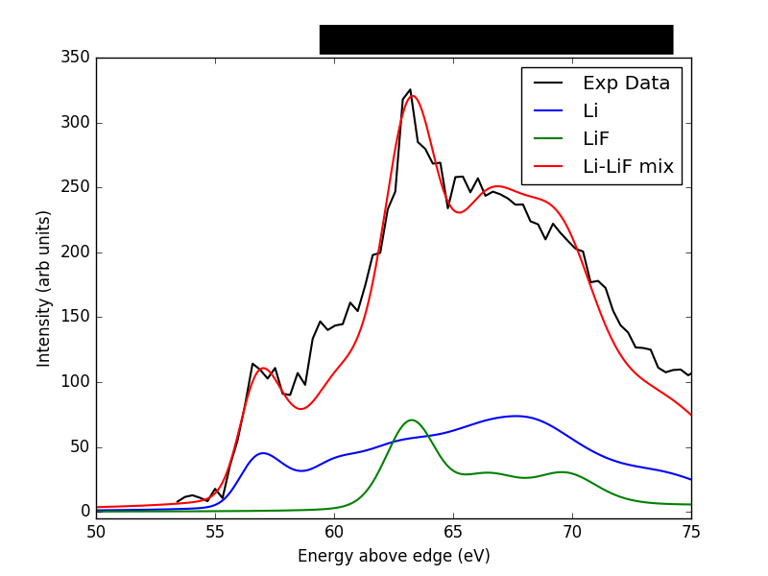
\includegraphics[width=1.1\textwidth]{Li-Lif_colour_unscreened}
		\caption{}
		\label{mix-unscreened}
	\end{subfigure}
	\caption{Lithium K edge of Li-LiF mix using full hole LiF spectrum and screened (a) and unscreened (b) metallic lithium spectrum. }

\label{Li-LiF_mix_screened}
\end{figure}



\section{Discussion}
The  cases analyzed above highlight the importance of including a core hole and screening effects when calculating ELNES of the lithium K edge.  In every case, a core hole was necessary, including metallic lithium which has been predicted to not exhibit core hole effects.  Additionally, every case except LiF exhibited non negligible amounts of screening  and applying the first order method developed in Chapter \ref{methods} results in dramatic improvements to experimental agreement.  The impact of including screening in ELNES calculations is made more apparent when dealing with unknown cases such as the Li-LiF mixture where it is essential to fingerprinting the near edge structure.  The improvement to the peak ratio in $ \mathrm{Li2O} $ is another key feature in terms of identifying oxidation on lithium edges, or taking the steps to quantitative analysis.  \\

Having improved upon the accuracy of the results, the effectiveness and applicability of the method is discussed below. The screening calculations do not depend on any additional empirical data relative to standard DFT.  Additionally, while three spectra are presented in each case for comparison (no hole, screened hole, and full hole), the technique predicts only a single correct result.  The current method in literature of choosing between hole or no hole introduces a degree of uncertainty, as multiple correct spectra are predicted for each case.   Any resulting disagreement can then be attributed to either screening effects or error. By only producing a single calculation which includes screening, this uncertainty is removed.  Another major benefit to the method is that it scales at the same rate as conventional DFT.  The largest computational cost occurs in the requirement to perform a third DFT calculations in order to obtain the screened result, an increase that scales at the same rate as the initial calculations.  Consequently, the method can be applied to any system that could be analyzed previously.  It is also of note, that the shielding calculations presented in this work are implemented in the cross section band structure one of the more lightweight first principle methods of calculating ELNES.\\

The success of the screening calculation when applied to lithium materials brings the generality of the approach into question.  As mentioned in Section \ref{calc_section}, core electron screening is ignored when calculating screening on the Li K edge.  For the K edges of heavier elements this component will increase, and be required when determining the valence electron screening.  As is, the method is largely limited to the lithium K edge.  The L/M edges of larger atoms may also see large improvements from this screening calculations, however, these cases become increasingly complex, as d-orbitals occupancy introduces a range of complications to the ELNES \cite{hubbard_electron_1963}. Consequently, in order to develop a approach to rapidly determine the screening coefficient in all cases, the core electron screening issue must be resolved.  \\


On a  final note, the reliable agreement between calculation and experiment helps solidify the validity of performing EELS at 30 keV to analyze beam sensitive materials.  The obtained experimental results were successful in reproducing agreement with the literature predictions when ignoring screening effects.  The ability to detect fine features such as the small second peak in metallic lithium and perform quantitative ratio analysis in $ \mathrm{Li_2O} $ emphasize the benefits of this method in analyzing beam sensitive materials.  \\








